\documentclass[a4paper, 12pt, italian]{report}
\usepackage{ctable}
\usepackage{url}
\usepackage[utf8]{inputenc}
\usepackage{graphicx}
\usepackage{amsmath}
\usepackage{usecases}
\usepackage[italian]{babel}

\usepackage[raggedright]{titlesec}
\usepackage{blindtext}

\titleformat{\chapter}[hang]{\bfseries\huge}{\thechapter.}{2pc}{}
\titlelabel{\thetitle.\quad}   % For consistency in all headings

\begin{document}
\begin{titlepage}
\newcommand{\HRule}{\rule{\linewidth}{0.5mm}} 
\center 
\textsc{\LARGE Università degli studi di Salerno}\\[1cm] 

\includegraphics[width=3.5cm]{img/logo.jpg} \\[1cm]
\textsc{\large Progetto di Ingegneria del Software II}\\[0.5cm]
\textsc{\Large Repominer Evolution}\\[0.5cm] 
 \HRule \\[0.4cm]
{ \large \bfseries Documento di manutenzione: analisi}\\[0.4cm] 
\HRule \\[1.5cm]

\begin{minipage}{0.4\textwidth}
\begin{flushleft} \large
\emph{Autori:}\\
Matteo \textsc{Merola}\\
Carlo \textsc{Branca}\\
Simone \textsc{Scalabrino}\\
Giovanni \textsc{Grano}\\
\end{flushleft}
\end{minipage}
~
\begin{minipage}{0.4\textwidth}
\begin{flushright} \large
\emph{Supervisore:} \\
Prof. Andrea \textsc{De Lucia}
\end{flushright}
\end{minipage}\\[2.5cm]

{\Large Documento di Manutenzione: analisi}\\
Versione 1.0\\[1cm]

{\large \today} % Date, change the \today to a set date if you want to be precise

\vfill

\end{titlepage}	
	\setcounter{tocdepth}{1}	
	\tableofcontents
	\listoffigures
	
	\chapter{Introduzione}

\section{Scopo del documento}
		
Il presente documento, oltre a fornire una panoramica del progetto, descrive il processo di management che sarà portato avanti durante le fasi progettazione e sviluppo. Il documento sarà aggiornato in maniera iterativa per offrire informazioni più precise riguardo le diverse fasi del progetto. 


\section{Evoluzione del presente documento}

Allo stato attuale del progetto, molte informazioni nel SPMP risultano incomplete o poco precise. Il documento sarà aggiornato e rivisto con l'avanzare dei lavori in modo da garantire una completa descrizione del processo manageriale condotto.


\section{Definizioni ed acronimi}

Definizioni:			
\begin{itemize}
\item \emph{Deliverables}: con il termine deliverables si ci riferisce generalmente alla documentazione tecnico/commerciale da consegnare al cliente quale risultato dell'esecuzione di una o più fasi di un progetto.
\item \emph{Scheduling}: pianificazione dei tempi e delle precedenze nell'impiego di risorse materiali ed umane per un buon svolgimento del processo di progettazione e sviluppo di un sistema software.
\item \emph{Work breakdown structure (WBS)}: rappresentazione di un progetto che consiste in una strutturazione tipicamente gerarchica delle attività che lo compongono in sotto-attività fino ad un opportuno livello di approfondimento.
\item \emph{Diagramma di Gantt}: strumento di supporto alla gestione dei progetti utilizzato principalmente nell'attività di project management quale rappresentazione dello scheduling delle attività o mansioni che costituiscono un progetto.
\end{itemize}	

Acronimi:
\begin{itemize}
\item \emph{ODD}: Object Design Document
\item \emph{WBS}: Work Breakdown Structure
\end{itemize}
	\chapter{Sistema proposto}
\section{Requisiti funzionali}
Il sistema deve essere in grado di calcolare metriche relative all'entropia di un progetto software.

Più in particolare, dovrà essere possibile calcolare le seguenti metriche basilari:
\begin{itemize}
\item Numero di revisioni del sistema;
\item Numero medio di volte in cui i file di un package hanno subito
cambiamenti;
\item Numero medio di volte in cui i file di un package hanno subito operazioni
di refactoring;
\item Numero medio di volte in cui i file di un package hanno subito operazioni di
bug fixing;
\item Numero di autori di commit effettuati all’interno di un package;
\item Numero di linee aggiunte o rimosse (somma, media e massimo);
\item Dimensione media dei file modificati.
\end{itemize}

Il sistema dovrà implementare il Basic Code Change Model descritto nell'articolo di Hassan \cite{hassan2009predicting}. Dovranno essere implementate, quindi, le seguenti metriche:
\begin{itemize}
\item Numero di cambiamenti totali di ogni file (righe aggiunte + righe cancellate) di un dato progetto software a seguito di aggiunta di feature (FI) in un periodo di riferimento (es: un mese); per distinguerle dovranno essere analizzati i messaggi di commit: quelli che non contengono parole come "bug-fix", "re-indent", "copyright update", etc. sono da classificare come FI.
\item Entropia dei cambiamenti dei file del progetto in un periodo di riferimento fissato (es: un mese)
\end{itemize}

Il sistema dovrà implementare l'Extended Code Change Model descritto nell'articolo di Hassan \cite{hassan2009predicting}; dovranno essere implementate, dunque, le seguenti metriche:

	\chapter{System Model}
\section{Use Case Models}

\subsection{UC\_QualityMetricsExtractor\_0.1}

	\begin{figure}[ht]
	\centering
	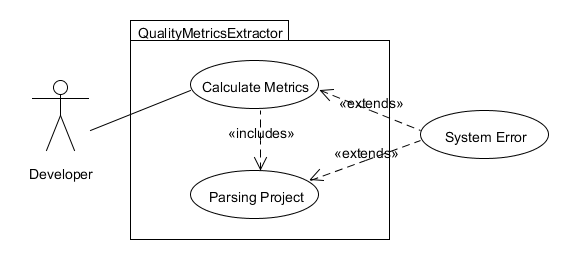
\includegraphics[scale=0.6]{img/usecase1.png}
	\caption{Use Case Diagram}\label{fig:usecase1}
	\end{figure}
\clearpage
%template caso d'uso
\begin{usecase}
\addtitle{Nome Use Case}{Calcolo metriche}
\addfield{ID:}{UC\_QualityMetricsExtractor\_0.1}
\addfield{Partecipanti:}{Sviluppatore}
\addfield{Condizioni di ingresso:}{Lo sviluppatore avvia la IDE "Eclipse"}
\addscenario{Flusso di eventi:}{
	\item Lo sviluppatore avvia il tool tramite il tasto "run".
	\item "SIE" apre una finestra della IDE mostrando sulla sinistra la lista dei progetti che è possibile analizzare.
	\item Lo sviluppatore seleziona il progetto, e da' avvio al programma.
	\item "SIE" notifica l'avvenuto calcolo delle metriche tramite un messaggio che compare in console.
}
\addfield{Condizioni di uscita:}{
	\begin{enumerate}
	\item[a.] Il sistema memorizza i dati.
	\item[b.] Lo sviluppatore termina precocemente l'operazione di calcolo.
	\end{enumerate}
}
\addfield{Eccezioni:}{Errore di sistema}
\end{usecase}

\clearpage
\subsection{UC\_ChangeConfigSettings}

	\begin{figure}[ht]
	\centering
	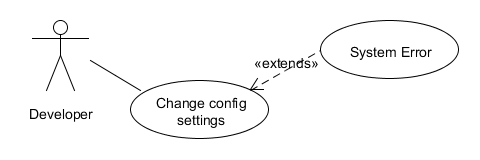
\includegraphics[scale=0.6]{img/usecase2.png}
	\caption{Use Case Diagram}\label{fig:usecase1}
	\end{figure}
	
\begin{usecase}
\addtitle{Nome Use Case}{Modifica file di configurazione}
\addfield{ID:}{UC\_ChangeConfigSettings}
\addfield{Partecipanti:}{Sviluppatore}
\addfield{Condizioni di ingresso:}{Il plugin è installato correttamente nell'IDE eclipse.}
\addscenario{Flusso di eventi:}{
	\item Lo sviluppatore apre il file settings.config con un qualsiasi editor di testo.
	\item Lo sviluppatore configura le metriche da calcolare.
}
\addfield{Condizioni di uscita:}{
	\begin{enumerate}
	\item[a.] Il plugin è configurato per le metriche desiderate.
	\item[b.] Lo sviluppatore ha scritto male i dati di configurazione.
	\end{enumerate}
}
\addfield{Eccezioni:}{Errore di sistema}
\end{usecase}

\section{Object Models}
La struttura dell'intero sistema software si sintetizza nel modello a oggetti rappresentato dal seguente diagramma.
\begin{figure}[ht]
	\centering
	%width=.5\textwidth
	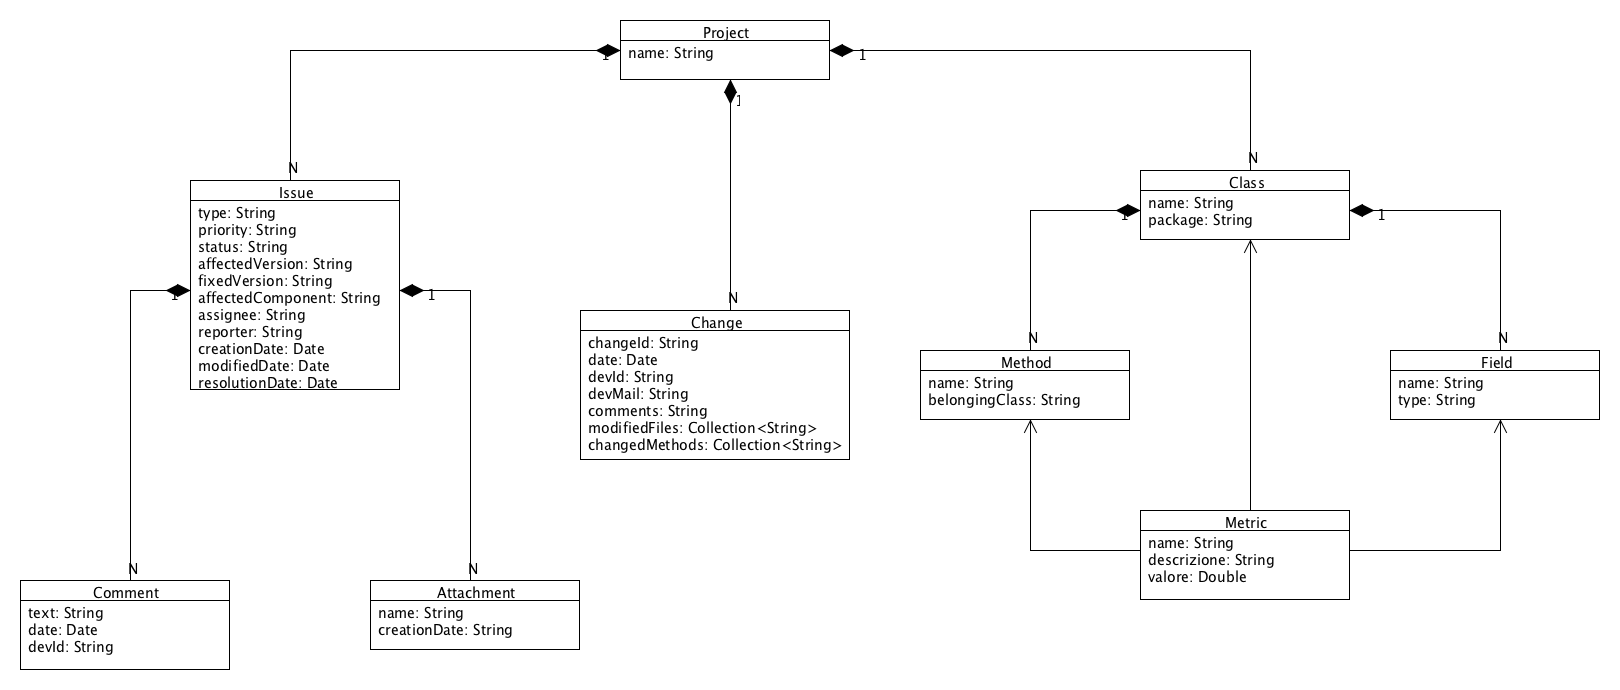
\includegraphics[width=1.1\textwidth, angle=90]{img/objectModel.png}
	\caption{Modello a oggetti}\label{fig:objectModel}
\end{figure}


	\chapter{Impact Analysis}
In questa sezione si presenterà una previsione dell'impatto che la modifica richiesta avrà sugli artefatti del sistema esistente. In particolar modo si cercherà di individuare le classi (codice sorgente) che dovranno essere modificate per integrare le funzionalità richieste.

\paragraph{}
Dato che si è scelto di implementare un sistema ex novo le cui funzionalità andranno ad affiancare e integrare quelle del sistema esistente, a livello di codice sorgente l'impatto sarà pari a zero.

RepominerEvo andrà ad interagire con esso solamente al layer di gestione dei dati, in quanto andrà a utilizzare le informazioni estrapolate e memorizzate da Repominer per implementare nuove funzionalità. Si può ragionevolmente dedurre quindi che l'impatto sul sistema esistente andrà gestito unicamente a livello di database.

Dato che dovranno essere implementate nuove metriche di natura più complessa ed articolata, si presume che sarà necessaria la modifica di alcune tabelle e di alcuni campi nel database esistente.
\\

Nella figura \ref{fig:sie} di pagina \pageref{fig:sie} riportiamo la relazioni e le tabelle più significative al momento corrente ai fini delle metriche da implementare.
\\
In particolare, ipotizziamo che lo Starting Impact Set conterrà la tabella:
\begin{itemize}
\item metrics
\end{itemize}
Si è pensato, dovendo estendere le metriche già calcolate in Repominer con nuove metriche, distinte in metriche di pacchetto e metriche di progetto, di dover prevedere la creazione di due nuove tabelle: 
\begin{itemize}
\item package\_metrics
\item project\_metrics
\end{itemize}

Nella figura \ref{fig:dettaglio} di pagina \pageref{fig:dettaglio} mostriamo le nuove relazioni ipotizzate che si verranno a creare. Si precisa che tali nuove relazioni non avranno alcuna influenza con la struttura del database preesistente.

\begin{figure}[t]
	\centering
	%width=.5\textwidth
	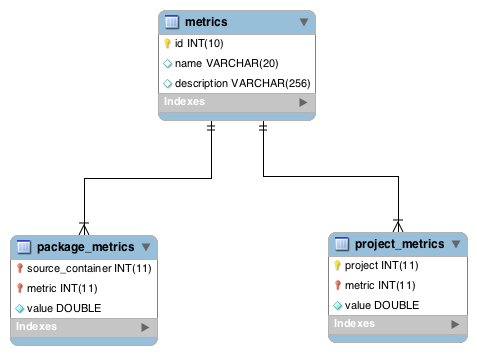
\includegraphics[width=.5\textwidth]{img/dettaglio.png}
	\caption{Nuove tabelle}\label{fig:dettaglio}
\end{figure}

\begin{figure}[b]
	\centering
	%width=.5\textwidth
	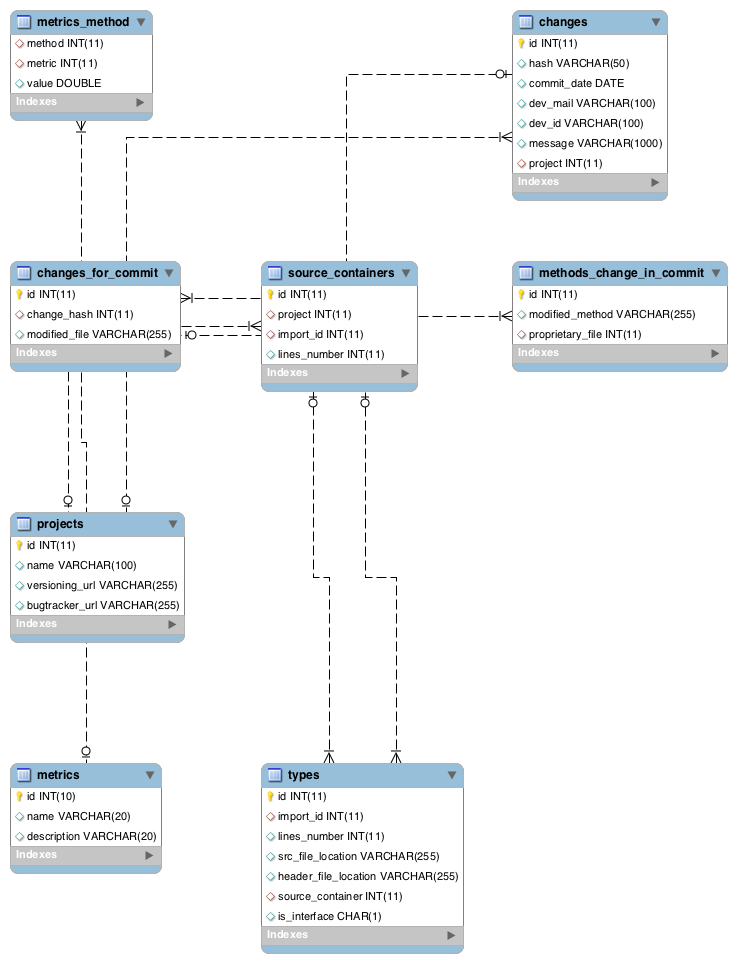
\includegraphics[width=\textwidth]{img/sieImportant.png}
	\caption{Dettaglio del DB con le relazioni principali}\label{fig:sie}
\end{figure}

A seguito di un'analisi approfondita, è stato individuato il Candidate Impact Set nell'unica tabella: 
\begin{itemize}
\item metrics
\end{itemize}
A seguito di tale analisi rimangono valide le considerazioni sopra esposte riguardo le nuove tabelle da creare e le relazioni da instaurare con \textit{metrics}.
\\

Una valutazione dettagliata dei risultati di questa analisi sarà presentata in un report separato dopo l'implementazione completa delle modifiche.
	%\chapter{Glossario}
	
\bibliography{bibliografia.bib}{}
\bibliographystyle{plain}
\end{document}
